% Options for packages loaded elsewhere
\PassOptionsToPackage{unicode}{hyperref}
\PassOptionsToPackage{hyphens}{url}
%
\documentclass[
]{article}
\usepackage{lmodern}
\usepackage{amssymb,amsmath}
\usepackage{ifxetex,ifluatex}
\ifnum 0\ifxetex 1\fi\ifluatex 1\fi=0 % if pdftex
  \usepackage[T1]{fontenc}
  \usepackage[utf8]{inputenc}
  \usepackage{textcomp} % provide euro and other symbols
\else % if luatex or xetex
  \usepackage{unicode-math}
  \defaultfontfeatures{Scale=MatchLowercase}
  \defaultfontfeatures[\rmfamily]{Ligatures=TeX,Scale=1}
\fi
% Use upquote if available, for straight quotes in verbatim environments
\IfFileExists{upquote.sty}{\usepackage{upquote}}{}
\IfFileExists{microtype.sty}{% use microtype if available
  \usepackage[]{microtype}
  \UseMicrotypeSet[protrusion]{basicmath} % disable protrusion for tt fonts
}{}
\makeatletter
\@ifundefined{KOMAClassName}{% if non-KOMA class
  \IfFileExists{parskip.sty}{%
    \usepackage{parskip}
  }{% else
    \setlength{\parindent}{0pt}
    \setlength{\parskip}{6pt plus 2pt minus 1pt}}
}{% if KOMA class
  \KOMAoptions{parskip=half}}
\makeatother
\usepackage{xcolor}
\IfFileExists{xurl.sty}{\usepackage{xurl}}{} % add URL line breaks if available
\IfFileExists{bookmark.sty}{\usepackage{bookmark}}{\usepackage{hyperref}}
\hypersetup{
  pdftitle={Labo 4.2: Régression linéaire :Violence},
  pdfauthor={Visseho Adjiwanou, PhD.},
  hidelinks,
  pdfcreator={LaTeX via pandoc}}
\urlstyle{same} % disable monospaced font for URLs
\usepackage[margin=1in]{geometry}
\usepackage{color}
\usepackage{fancyvrb}
\newcommand{\VerbBar}{|}
\newcommand{\VERB}{\Verb[commandchars=\\\{\}]}
\DefineVerbatimEnvironment{Highlighting}{Verbatim}{commandchars=\\\{\}}
% Add ',fontsize=\small' for more characters per line
\usepackage{framed}
\definecolor{shadecolor}{RGB}{248,248,248}
\newenvironment{Shaded}{\begin{snugshade}}{\end{snugshade}}
\newcommand{\AlertTok}[1]{\textcolor[rgb]{0.94,0.16,0.16}{#1}}
\newcommand{\AnnotationTok}[1]{\textcolor[rgb]{0.56,0.35,0.01}{\textbf{\textit{#1}}}}
\newcommand{\AttributeTok}[1]{\textcolor[rgb]{0.77,0.63,0.00}{#1}}
\newcommand{\BaseNTok}[1]{\textcolor[rgb]{0.00,0.00,0.81}{#1}}
\newcommand{\BuiltInTok}[1]{#1}
\newcommand{\CharTok}[1]{\textcolor[rgb]{0.31,0.60,0.02}{#1}}
\newcommand{\CommentTok}[1]{\textcolor[rgb]{0.56,0.35,0.01}{\textit{#1}}}
\newcommand{\CommentVarTok}[1]{\textcolor[rgb]{0.56,0.35,0.01}{\textbf{\textit{#1}}}}
\newcommand{\ConstantTok}[1]{\textcolor[rgb]{0.00,0.00,0.00}{#1}}
\newcommand{\ControlFlowTok}[1]{\textcolor[rgb]{0.13,0.29,0.53}{\textbf{#1}}}
\newcommand{\DataTypeTok}[1]{\textcolor[rgb]{0.13,0.29,0.53}{#1}}
\newcommand{\DecValTok}[1]{\textcolor[rgb]{0.00,0.00,0.81}{#1}}
\newcommand{\DocumentationTok}[1]{\textcolor[rgb]{0.56,0.35,0.01}{\textbf{\textit{#1}}}}
\newcommand{\ErrorTok}[1]{\textcolor[rgb]{0.64,0.00,0.00}{\textbf{#1}}}
\newcommand{\ExtensionTok}[1]{#1}
\newcommand{\FloatTok}[1]{\textcolor[rgb]{0.00,0.00,0.81}{#1}}
\newcommand{\FunctionTok}[1]{\textcolor[rgb]{0.00,0.00,0.00}{#1}}
\newcommand{\ImportTok}[1]{#1}
\newcommand{\InformationTok}[1]{\textcolor[rgb]{0.56,0.35,0.01}{\textbf{\textit{#1}}}}
\newcommand{\KeywordTok}[1]{\textcolor[rgb]{0.13,0.29,0.53}{\textbf{#1}}}
\newcommand{\NormalTok}[1]{#1}
\newcommand{\OperatorTok}[1]{\textcolor[rgb]{0.81,0.36,0.00}{\textbf{#1}}}
\newcommand{\OtherTok}[1]{\textcolor[rgb]{0.56,0.35,0.01}{#1}}
\newcommand{\PreprocessorTok}[1]{\textcolor[rgb]{0.56,0.35,0.01}{\textit{#1}}}
\newcommand{\RegionMarkerTok}[1]{#1}
\newcommand{\SpecialCharTok}[1]{\textcolor[rgb]{0.00,0.00,0.00}{#1}}
\newcommand{\SpecialStringTok}[1]{\textcolor[rgb]{0.31,0.60,0.02}{#1}}
\newcommand{\StringTok}[1]{\textcolor[rgb]{0.31,0.60,0.02}{#1}}
\newcommand{\VariableTok}[1]{\textcolor[rgb]{0.00,0.00,0.00}{#1}}
\newcommand{\VerbatimStringTok}[1]{\textcolor[rgb]{0.31,0.60,0.02}{#1}}
\newcommand{\WarningTok}[1]{\textcolor[rgb]{0.56,0.35,0.01}{\textbf{\textit{#1}}}}
\usepackage{longtable,booktabs}
% Correct order of tables after \paragraph or \subparagraph
\usepackage{etoolbox}
\makeatletter
\patchcmd\longtable{\par}{\if@noskipsec\mbox{}\fi\par}{}{}
\makeatother
% Allow footnotes in longtable head/foot
\IfFileExists{footnotehyper.sty}{\usepackage{footnotehyper}}{\usepackage{footnote}}
\makesavenoteenv{longtable}
\usepackage{graphicx,grffile}
\makeatletter
\def\maxwidth{\ifdim\Gin@nat@width>\linewidth\linewidth\else\Gin@nat@width\fi}
\def\maxheight{\ifdim\Gin@nat@height>\textheight\textheight\else\Gin@nat@height\fi}
\makeatother
% Scale images if necessary, so that they will not overflow the page
% margins by default, and it is still possible to overwrite the defaults
% using explicit options in \includegraphics[width, height, ...]{}
\setkeys{Gin}{width=\maxwidth,height=\maxheight,keepaspectratio}
% Set default figure placement to htbp
\makeatletter
\def\fps@figure{htbp}
\makeatother
\setlength{\emergencystretch}{3em} % prevent overfull lines
\providecommand{\tightlist}{%
  \setlength{\itemsep}{0pt}\setlength{\parskip}{0pt}}
\setcounter{secnumdepth}{-\maxdimen} % remove section numbering

\title{Labo 4.2: Régression linéaire :Violence}
\author{Visseho Adjiwanou, PhD.}
\date{10 June 2021}

\begin{document}
\maketitle

\hypertarget{exemple-1}{%
\subsection{Exemple 1:}\label{exemple-1}}

Présenter à nouveau la discussion sur la relation entre violence
conjugale et l'accès à l'information mesurée par les variables
\texttt{sec\_school} et \texttt{no\_media}. ouverture aux médias
éducation et radio

\hypertarget{exemple}{%
\subsection{Exemple}\label{exemple}}

\begin{longtable}[]{@{}ll@{}}
\toprule
Name & Description\tabularnewline
\midrule
\endhead
\texttt{beat\_goesout} & Pourcentage de femmes dans chaque pays qui
pensent qu'un mari\tabularnewline
& a le droit de battre sa femme si elle sort sans le lui
dire.\tabularnewline
\texttt{beat\_burnfood} & Pourcentage de femmes dans chaque pays qui
pensent qu'un mari\tabularnewline
& a le droit de battre sa femme si elle brûle sa
nourriture.\tabularnewline
\texttt{no\_media} & Pourcentage de femmes dans chaque pays qui ont
rarement accès\tabularnewline
& un journal, une radio ou une télévision.\tabularnewline
\texttt{sec\_school} & Pourcentage de femmes dans chaque pays ayant un
niveau\tabularnewline
& d'éducation secondaire ou supérieur.\tabularnewline
\texttt{year} & Année de l'enquête\tabularnewline
\texttt{region} & Région du monde\tabularnewline
\texttt{country} & pays\tabularnewline
\bottomrule
\end{longtable}

\begin{Shaded}
\begin{Highlighting}[]
\KeywordTok{rm}\NormalTok{(}\DataTypeTok{list =} \KeywordTok{ls}\NormalTok{())}

\CommentTok{#install.packages("broom")}

\KeywordTok{library}\NormalTok{(tidyverse)}
\end{Highlighting}
\end{Shaded}

\begin{verbatim}
## -- Attaching packages --------------------------------------- tidyverse 1.3.0 --
\end{verbatim}

\begin{verbatim}
## v ggplot2 3.3.3     v purrr   0.3.4
## v tibble  3.0.6     v dplyr   1.0.4
## v tidyr   1.1.2     v stringr 1.4.0
## v readr   1.4.0     v forcats 0.5.1
\end{verbatim}

\begin{verbatim}
## Warning: package 'ggplot2' was built under R version 3.6.2
\end{verbatim}

\begin{verbatim}
## Warning: package 'tibble' was built under R version 3.6.2
\end{verbatim}

\begin{verbatim}
## Warning: package 'tidyr' was built under R version 3.6.2
\end{verbatim}

\begin{verbatim}
## Warning: package 'readr' was built under R version 3.6.2
\end{verbatim}

\begin{verbatim}
## Warning: package 'purrr' was built under R version 3.6.2
\end{verbatim}

\begin{verbatim}
## Warning: package 'dplyr' was built under R version 3.6.2
\end{verbatim}

\begin{verbatim}
## Warning: package 'forcats' was built under R version 3.6.2
\end{verbatim}

\begin{verbatim}
## -- Conflicts ------------------------------------------ tidyverse_conflicts() --
## x dplyr::filter() masks stats::filter()
## x dplyr::lag()    masks stats::lag()
\end{verbatim}

\begin{Shaded}
\begin{Highlighting}[]
\KeywordTok{library}\NormalTok{(summarytools)}
\end{Highlighting}
\end{Shaded}

\begin{verbatim}
## Registered S3 method overwritten by 'pryr':
##   method      from
##   print.bytes Rcpp
\end{verbatim}

\begin{verbatim}
## Warning in system2("/usr/bin/otool", c("-L", shQuote(DSO)), stdout = TRUE):
## running command ''/usr/bin/otool' -L '/Library/Frameworks/R.framework/Resources/
## library/tcltk/libs//tcltk.so'' had status 1
\end{verbatim}

\begin{verbatim}
## For best results, restart R session and update pander using devtools:: or remotes::install_github('rapporter/pander')
\end{verbatim}

\begin{verbatim}
## 
## Attaching package: 'summarytools'
\end{verbatim}

\begin{verbatim}
## The following object is masked from 'package:tibble':
## 
##     view
\end{verbatim}

\begin{Shaded}
\begin{Highlighting}[]
\KeywordTok{library}\NormalTok{(broom)}
\end{Highlighting}
\end{Shaded}

\begin{verbatim}
## Warning: package 'broom' was built under R version 3.6.2
\end{verbatim}

\begin{Shaded}
\begin{Highlighting}[]
\NormalTok{dhs_ipv <-}\StringTok{ }\KeywordTok{read_csv}\NormalTok{(}\StringTok{"../Données/dhs_ipv.csv"}\NormalTok{)}
\end{Highlighting}
\end{Shaded}

\begin{verbatim}
## Warning: Missing column names filled in: 'X1' [1]
\end{verbatim}

\begin{verbatim}
## 
## -- Column specification --------------------------------------------------------
## cols(
##   X1 = col_double(),
##   beat_burnfood = col_double(),
##   beat_goesout = col_double(),
##   sec_school = col_double(),
##   no_media = col_double(),
##   country = col_character(),
##   year = col_double(),
##   region = col_character()
## )
\end{verbatim}

\begin{Shaded}
\begin{Highlighting}[]
\KeywordTok{summary}\NormalTok{(dhs_ipv)}
\end{Highlighting}
\end{Shaded}

\begin{verbatim}
##        X1         beat_burnfood    beat_goesout     sec_school   
##  Min.   :  1.00   Min.   : 0.10   Min.   : 0.30   Min.   : 3.10  
##  1st Qu.: 40.50   1st Qu.: 4.50   1st Qu.:11.85   1st Qu.:10.18  
##  Median : 79.00   Median :11.85   Median :28.10   Median :22.40  
##  Mean   : 80.53   Mean   :15.04   Mean   :28.60   Mean   :24.40  
##  3rd Qu.:119.50   3rd Qu.:22.25   3rd Qu.:42.08   3rd Qu.:34.90  
##  Max.   :160.00   Max.   :64.50   Max.   :82.70   Max.   :74.60  
##                   NA's   :31      NA's   :27      NA's   :3      
##     no_media       country               year         region         
##  Min.   : 0.80   Length:151         Min.   :1999   Length:151        
##  1st Qu.:11.25   Class :character   1st Qu.:2004   Class :character  
##  Median :29.15   Mode  :character   Median :2007   Mode  :character  
##  Mean   :28.40                      Mean   :2007                     
##  3rd Qu.:43.23                      3rd Qu.:2011                     
##  Max.   :86.40                      Max.   :2014                     
##  NA's   :13
\end{verbatim}

\hypertarget{ruxe9gression-linuxe9aire-simple}{%
\section{Régression linéaire
simple}\label{ruxe9gression-linuxe9aire-simple}}

\hypertarget{effet-du-niveau-de-scolarisation-sur-lattitude-face-uxe0-la-violence}{%
\subsection{Effet du niveau de scolarisation sur l'attitude face à la
violence}\label{effet-du-niveau-de-scolarisation-sur-lattitude-face-uxe0-la-violence}}

\begin{Shaded}
\begin{Highlighting}[]
\KeywordTok{class}\NormalTok{(dhs_ipv}\OperatorTok{$}\NormalTok{beat_burnfood)}
\end{Highlighting}
\end{Shaded}

\begin{verbatim}
## [1] "numeric"
\end{verbatim}

\begin{Shaded}
\begin{Highlighting}[]
\KeywordTok{lm}\NormalTok{(beat_burnfood }\OperatorTok{~}\StringTok{ }\NormalTok{sec_school, }\DataTypeTok{data =}\NormalTok{ dhs_ipv)}
\end{Highlighting}
\end{Shaded}

\begin{verbatim}
## 
## Call:
## lm(formula = beat_burnfood ~ sec_school, data = dhs_ipv)
## 
## Coefficients:
## (Intercept)   sec_school  
##     24.0703      -0.3868
\end{verbatim}

Comment interprétez-vous ces résultats?

\textbf{Interprétation}

Une augmentation d'une unité du pourcentage de femmes ayant le niveau
secondaire ou plus entraîne une diminution de 0,38 soit de 38\% du
pourcentage des femmes qui estiment qu'une femme doit être battue si
elle brûle la nourriture.

De manière générale, on dit:

Une augmentation d'une unité de la \textbf{variable indépendante}
entraîne une augmentation/diminution de \(\beta\) de la \textbf{variable
dépendante}

\hypertarget{formes-du-ruxe9sultats}{%
\subsection{Formes du résultats}\label{formes-du-ruxe9sultats}}

\begin{Shaded}
\begin{Highlighting}[]
\NormalTok{reg1 <-}\StringTok{ }\KeywordTok{lm}\NormalTok{(beat_burnfood }\OperatorTok{~}\StringTok{ }\NormalTok{sec_school, }\DataTypeTok{data =}\NormalTok{ dhs_ipv)}
\NormalTok{reg1}
\end{Highlighting}
\end{Shaded}

\begin{verbatim}
## 
## Call:
## lm(formula = beat_burnfood ~ sec_school, data = dhs_ipv)
## 
## Coefficients:
## (Intercept)   sec_school  
##     24.0703      -0.3868
\end{verbatim}

\begin{Shaded}
\begin{Highlighting}[]
\CommentTok{# ou}

\KeywordTok{coef}\NormalTok{(reg1)}
\end{Highlighting}
\end{Shaded}

\begin{verbatim}
## (Intercept)  sec_school 
##  24.0702721  -0.3868353
\end{verbatim}

\hypertarget{des-ruxe9sultats-plus-duxe9tailluxe9s}{%
\subsection{Des résultats plus
détaillés}\label{des-ruxe9sultats-plus-duxe9tailluxe9s}}

\begin{Shaded}
\begin{Highlighting}[]
\KeywordTok{summary}\NormalTok{(reg1)}
\end{Highlighting}
\end{Shaded}

\begin{verbatim}
## 
## Call:
## lm(formula = beat_burnfood ~ sec_school, data = dhs_ipv)
## 
## Residuals:
##     Min      1Q  Median      3Q     Max 
## -15.857  -8.786  -1.870   3.618  42.364 
## 
## Coefficients:
##             Estimate Std. Error t value Pr(>|t|)    
## (Intercept) 24.07027    1.91920  12.542  < 2e-16 ***
## sec_school  -0.38684    0.06634  -5.831 5.07e-08 ***
## ---
## Signif. codes:  0 '***' 0.001 '**' 0.01 '*' 0.05 '.' 0.1 ' ' 1
## 
## Residual standard error: 11.43 on 116 degrees of freedom
##   (33 observations deleted due to missingness)
## Multiple R-squared:  0.2267, Adjusted R-squared:   0.22 
## F-statistic:    34 on 1 and 116 DF,  p-value: 5.069e-08
\end{verbatim}

\hypertarget{relation-entre-beat_burnfood-et-le-non-accuxe8s-aux-muxe9dias}{%
\subsection{Relation entre beat\_burnfood et le non-accès aux
médias}\label{relation-entre-beat_burnfood-et-le-non-accuxe8s-aux-muxe9dias}}

\begin{Shaded}
\begin{Highlighting}[]
\NormalTok{reg2 <-}\StringTok{ }\KeywordTok{lm}\NormalTok{(beat_burnfood }\OperatorTok{~}\StringTok{  }\NormalTok{no_media, }\DataTypeTok{data =}\NormalTok{ dhs_ipv)}
\KeywordTok{summary}\NormalTok{(reg2)}
\end{Highlighting}
\end{Shaded}

\begin{verbatim}
## 
## Call:
## lm(formula = beat_burnfood ~ no_media, data = dhs_ipv)
## 
## Residuals:
##     Min      1Q  Median      3Q     Max 
## -19.637  -6.581  -2.188   4.316  51.913 
## 
## Coefficients:
##             Estimate Std. Error t value Pr(>|t|)    
## (Intercept)   3.5289     1.7728   1.991   0.0489 *  
## no_media      0.4141     0.0517   8.010 9.93e-13 ***
## ---
## Signif. codes:  0 '***' 0.001 '**' 0.01 '*' 0.05 '.' 0.1 ' ' 1
## 
## Residual standard error: 10.87 on 116 degrees of freedom
##   (33 observations deleted due to missingness)
## Multiple R-squared:  0.3561, Adjusted R-squared:  0.3506 
## F-statistic: 64.16 on 1 and 116 DF,  p-value: 9.932e-13
\end{verbatim}

\hypertarget{relation-entre-beat_burnfood-et-la-ruxe9gion}{%
\subsection{Relation entre beat\_burnfood et la
région}\label{relation-entre-beat_burnfood-et-la-ruxe9gion}}

\begin{Shaded}
\begin{Highlighting}[]
\KeywordTok{class}\NormalTok{(dhs_ipv}\OperatorTok{$}\NormalTok{region)}
\end{Highlighting}
\end{Shaded}

\begin{verbatim}
## [1] "character"
\end{verbatim}

\begin{Shaded}
\begin{Highlighting}[]
\KeywordTok{freq}\NormalTok{(dhs_ipv}\OperatorTok{$}\NormalTok{region)}
\end{Highlighting}
\end{Shaded}

\begin{verbatim}
## Frequencies  
## dhs_ipv$region  
## Type: Character  
## 
##                                      Freq   % Valid   % Valid Cum.   % Total   % Total Cum.
## ---------------------------------- ------ --------- -------------- --------- --------------
##                               Asia     24     15.89          15.89     15.89          15.89
##                      Latin America     24     15.89          31.79     15.89          31.79
##       Middle East and Central Asia     19     12.58          44.37     12.58          44.37
##                 Sub-Saharan Africa     84     55.63         100.00     55.63         100.00
##                               <NA>      0                               0.00         100.00
##                              Total    151    100.00         100.00    100.00         100.00
\end{verbatim}

\begin{Shaded}
\begin{Highlighting}[]
\NormalTok{reg3 <-}\StringTok{ }\KeywordTok{lm}\NormalTok{(beat_burnfood }\OperatorTok{~}\StringTok{  }\NormalTok{region, }\DataTypeTok{data =}\NormalTok{ dhs_ipv)}
\NormalTok{reg3}
\end{Highlighting}
\end{Shaded}

\begin{verbatim}
## 
## Call:
## lm(formula = beat_burnfood ~ region, data = dhs_ipv)
## 
## Coefficients:
##                        (Intercept)                 regionLatin America  
##                              8.306                              -4.611  
## regionMiddle East and Central Asia            regionSub-Saharan Africa  
##                              3.713                              12.554
\end{verbatim}

\begin{Shaded}
\begin{Highlighting}[]
\KeywordTok{summary}\NormalTok{(reg3)}
\end{Highlighting}
\end{Shaded}

\begin{verbatim}
## 
## Call:
## lm(formula = beat_burnfood ~ region, data = dhs_ipv)
## 
## Residuals:
##     Min      1Q  Median      3Q     Max 
## -16.360  -7.154  -2.527   3.565  47.481 
## 
## Coefficients:
##                                    Estimate Std. Error t value Pr(>|t|)    
## (Intercept)                           8.306      2.834   2.931 0.004075 ** 
## regionLatin America                  -4.611      3.855  -1.196 0.234087    
## regionMiddle East and Central Asia    3.713      4.070   0.912 0.363554    
## regionSub-Saharan Africa             12.554      3.173   3.956 0.000132 ***
## ---
## Signif. codes:  0 '***' 0.001 '**' 0.01 '*' 0.05 '.' 0.1 ' ' 1
## 
## Residual standard error: 11.69 on 116 degrees of freedom
##   (31 observations deleted due to missingness)
## Multiple R-squared:  0.2667, Adjusted R-squared:  0.2477 
## F-statistic: 14.06 on 3 and 116 DF,  p-value: 7.026e-08
\end{verbatim}

\hypertarget{relation-entre-beat_burnfood-et-lannuxe9e}{%
\subsection{Relation entre beat\_burnfood et
l'année}\label{relation-entre-beat_burnfood-et-lannuxe9e}}

\begin{Shaded}
\begin{Highlighting}[]
\KeywordTok{class}\NormalTok{(dhs_ipv}\OperatorTok{$}\NormalTok{year)}
\end{Highlighting}
\end{Shaded}

\begin{verbatim}
## [1] "numeric"
\end{verbatim}

\begin{Shaded}
\begin{Highlighting}[]
\NormalTok{dhs_ipv <-}
\StringTok{  }\NormalTok{dhs_ipv }\OperatorTok\StringTok{ }
\StringTok{  }\KeywordTok{mutate}\NormalTok{(}\DataTypeTok{year_binaire =} \KeywordTok{factor}\NormalTok{(}\KeywordTok{if_else}\NormalTok{(year }\OperatorTok{<=}\StringTok{ }\DecValTok{2010}\NormalTok{, }\StringTok{"Avant 2010"}\NormalTok{, }\StringTok{"Apres 2010"}\NormalTok{)))}

\KeywordTok{freq}\NormalTok{(dhs_ipv}\OperatorTok{$}\NormalTok{year_binaire)}
\end{Highlighting}
\end{Shaded}

\begin{verbatim}
## Frequencies  
## dhs_ipv$year_binaire  
## Type: Factor  
## 
##                    Freq   % Valid   % Valid Cum.   % Total   % Total Cum.
## ---------------- ------ --------- -------------- --------- --------------
##       Apres 2010     41     27.15          27.15     27.15          27.15
##       Avant 2010    110     72.85         100.00     72.85         100.00
##             <NA>      0                               0.00         100.00
##            Total    151    100.00         100.00    100.00         100.00
\end{verbatim}

\begin{Shaded}
\begin{Highlighting}[]
\NormalTok{reg4 <-}\StringTok{ }\KeywordTok{lm}\NormalTok{(beat_burnfood }\OperatorTok{~}\StringTok{  }\NormalTok{year_binaire, }\DataTypeTok{data =}\NormalTok{ dhs_ipv)}
\KeywordTok{summary}\NormalTok{(reg4)}
\end{Highlighting}
\end{Shaded}

\begin{verbatim}
## 
## Call:
## lm(formula = beat_burnfood ~ year_binaire, data = dhs_ipv)
## 
## Residuals:
##     Min      1Q  Median      3Q     Max 
## -15.649 -10.449  -3.249   6.647  48.751 
## 
## Coefficients:
##                        Estimate Std. Error t value Pr(>|t|)    
## (Intercept)              13.454      2.217   6.068 1.61e-08 ***
## year_binaireAvant 2010    2.295      2.666   0.861    0.391    
## ---
## Signif. codes:  0 '***' 0.001 '**' 0.01 '*' 0.05 '.' 0.1 ' ' 1
## 
## Residual standard error: 13.49 on 118 degrees of freedom
##   (31 observations deleted due to missingness)
## Multiple R-squared:  0.006242,   Adjusted R-squared:  -0.002179 
## F-statistic: 0.7412 on 1 and 118 DF,  p-value: 0.391
\end{verbatim}

\hypertarget{changement-de-la-catuxe9gorie-de-ruxe9fuxe9rence}{%
\subsection{Changement de la catégorie de
référence}\label{changement-de-la-catuxe9gorie-de-ruxe9fuxe9rence}}

\url{https://stackoverflow.com/questions/3872070/how-to-force-r-to-use-a-specified-factor-level-as-reference-in-a-regression}

\begin{Shaded}
\begin{Highlighting}[]
\NormalTok{?relevel}

\NormalTok{reg5 <-}\StringTok{ }\KeywordTok{lm}\NormalTok{(beat_burnfood }\OperatorTok{~}\StringTok{ }\KeywordTok{relevel}\NormalTok{(year_binaire, }\DataTypeTok{ref =} \StringTok{"Avant 2010"}\NormalTok{), }\DataTypeTok{data =}\NormalTok{ dhs_ipv)}
\KeywordTok{coef}\NormalTok{(reg5)}
\end{Highlighting}
\end{Shaded}

\begin{verbatim}
##                                         (Intercept) 
##                                           15.749398 
## relevel(year_binaire, ref = "Avant 2010")Apres 2010 
##                                           -2.295344
\end{verbatim}

\begin{Shaded}
\begin{Highlighting}[]
\NormalTok{dhs_ipv <-}
\StringTok{  }\NormalTok{dhs_ipv }\OperatorTok\StringTok{ }
\StringTok{  }\KeywordTok{mutate}\NormalTok{(}\DataTypeTok{year_binaire1 =} \KeywordTok{factor}\NormalTok{(}\KeywordTok{if_else}\NormalTok{(year }\OperatorTok{<=}\StringTok{ }\DecValTok{2010}\NormalTok{, }\StringTok{"Avant 2010"}\NormalTok{, }\StringTok{"Apres 2010"}\NormalTok{), }\DataTypeTok{levels =} \KeywordTok{c}\NormalTok{(}\StringTok{"Avant 2010"}\NormalTok{, }\StringTok{"Apres 2010"}\NormalTok{)))}

\KeywordTok{freq}\NormalTok{(dhs_ipv}\OperatorTok{$}\NormalTok{year_binaire1)}
\end{Highlighting}
\end{Shaded}

\begin{verbatim}
## Frequencies  
## dhs_ipv$year_binaire1  
## Type: Factor  
## 
##                    Freq   % Valid   % Valid Cum.   % Total   % Total Cum.
## ---------------- ------ --------- -------------- --------- --------------
##       Avant 2010    110     72.85          72.85     72.85          72.85
##       Apres 2010     41     27.15         100.00     27.15         100.00
##             <NA>      0                               0.00         100.00
##            Total    151    100.00         100.00    100.00         100.00
\end{verbatim}

\begin{Shaded}
\begin{Highlighting}[]
\NormalTok{reg6 <-}\StringTok{ }\KeywordTok{lm}\NormalTok{(beat_burnfood }\OperatorTok{~}\StringTok{  }\NormalTok{year_binaire1, }\DataTypeTok{data =}\NormalTok{ dhs_ipv)}
\KeywordTok{summary}\NormalTok{(reg6)}
\end{Highlighting}
\end{Shaded}

\begin{verbatim}
## 
## Call:
## lm(formula = beat_burnfood ~ year_binaire1, data = dhs_ipv)
## 
## Residuals:
##     Min      1Q  Median      3Q     Max 
## -15.649 -10.449  -3.249   6.647  48.751 
## 
## Coefficients:
##                         Estimate Std. Error t value Pr(>|t|)    
## (Intercept)               15.749      1.480  10.638   <2e-16 ***
## year_binaire1Apres 2010   -2.295      2.666  -0.861    0.391    
## ---
## Signif. codes:  0 '***' 0.001 '**' 0.01 '*' 0.05 '.' 0.1 ' ' 1
## 
## Residual standard error: 13.49 on 118 degrees of freedom
##   (31 observations deleted due to missingness)
## Multiple R-squared:  0.006242,   Adjusted R-squared:  -0.002179 
## F-statistic: 0.7412 on 1 and 118 DF,  p-value: 0.391
\end{verbatim}

\hypertarget{ruxe9gression-multiple}{%
\section{Régression multiple}\label{ruxe9gression-multiple}}

\hypertarget{relation-entre-attitude-face-a-la-violence-et-ouverture}{%
\subsection{Relation entre attitude face a la violence et
ouverture}\label{relation-entre-attitude-face-a-la-violence-et-ouverture}}

\begin{Shaded}
\begin{Highlighting}[]
\NormalTok{reg_mul1 <-}\StringTok{ }\KeywordTok{lm}\NormalTok{(beat_burnfood }\OperatorTok{~}\StringTok{ }\NormalTok{sec_school }\OperatorTok{+}\StringTok{ }\NormalTok{no_media, }\DataTypeTok{data =}\NormalTok{ dhs_ipv)}
\NormalTok{reg_mul1}
\end{Highlighting}
\end{Shaded}

\begin{verbatim}
## 
## Call:
## lm(formula = beat_burnfood ~ sec_school + no_media, data = dhs_ipv)
## 
## Coefficients:
## (Intercept)   sec_school     no_media  
##      6.4089      -0.1027       0.3850
\end{verbatim}

\begin{Shaded}
\begin{Highlighting}[]
\KeywordTok{summary}\NormalTok{(reg_mul1)}
\end{Highlighting}
\end{Shaded}

\begin{verbatim}
## 
## Call:
## lm(formula = beat_burnfood ~ sec_school + no_media, data = dhs_ipv)
## 
## Residuals:
##     Min      1Q  Median      3Q     Max 
## -18.405  -6.138  -1.813   4.553  25.342 
## 
## Coefficients:
##             Estimate Std. Error t value Pr(>|t|)    
## (Intercept)  6.40892    3.19095   2.008    0.047 *  
## sec_school  -0.10266    0.07182  -1.429    0.156    
## no_media     0.38499    0.05873   6.555 1.73e-09 ***
## ---
## Signif. codes:  0 '***' 0.001 '**' 0.01 '*' 0.05 '.' 0.1 ' ' 1
## 
## Residual standard error: 9.759 on 113 degrees of freedom
##   (35 observations deleted due to missingness)
## Multiple R-squared:  0.4416, Adjusted R-squared:  0.4317 
## F-statistic: 44.67 on 2 and 113 DF,  p-value: 5.063e-15
\end{verbatim}

\begin{Shaded}
\begin{Highlighting}[]
\KeywordTok{cor}\NormalTok{(dhs_ipv}\OperatorTok{$}\NormalTok{sec_school, dhs_ipv}\OperatorTok{$}\NormalTok{no_media, }\DataTypeTok{use =} \StringTok{"pairwise.complete.obs"}\NormalTok{)}
\end{Highlighting}
\end{Shaded}

\begin{verbatim}
## [1] -0.6077951
\end{verbatim}

\begin{Shaded}
\begin{Highlighting}[]
\NormalTok{?cor}
\end{Highlighting}
\end{Shaded}

\textbf{Interprétation}

\textbf{Toute choses étant égales par ailleurs (\emph{ceteris
paribus})}, une augmentation d'une unité du pourcentage de femmes ayant
le niveau secondaire ou plus entraîne une diminution de 0,103 soit de
10\% du pourcentage des femmes qui estiment qu'une femme doit être
battue si elle brûle la nourriture.

Pourquoi l'effet de l'éducation avait baissé? On avait trouvé avant une
diminution de 38\%.

Il faut regarder dans les hypothèses, celles qui peut avoir causer cela.

\begin{Shaded}
\begin{Highlighting}[]
\NormalTok{knitr}\OperatorTok{::}\KeywordTok{include_graphics}\NormalTok{(}\StringTok{"/Users/visseho/OneDrive - UQAM/Cours/Images_cours/hypotheses_regression.png"}\NormalTok{)}
\end{Highlighting}
\end{Shaded}

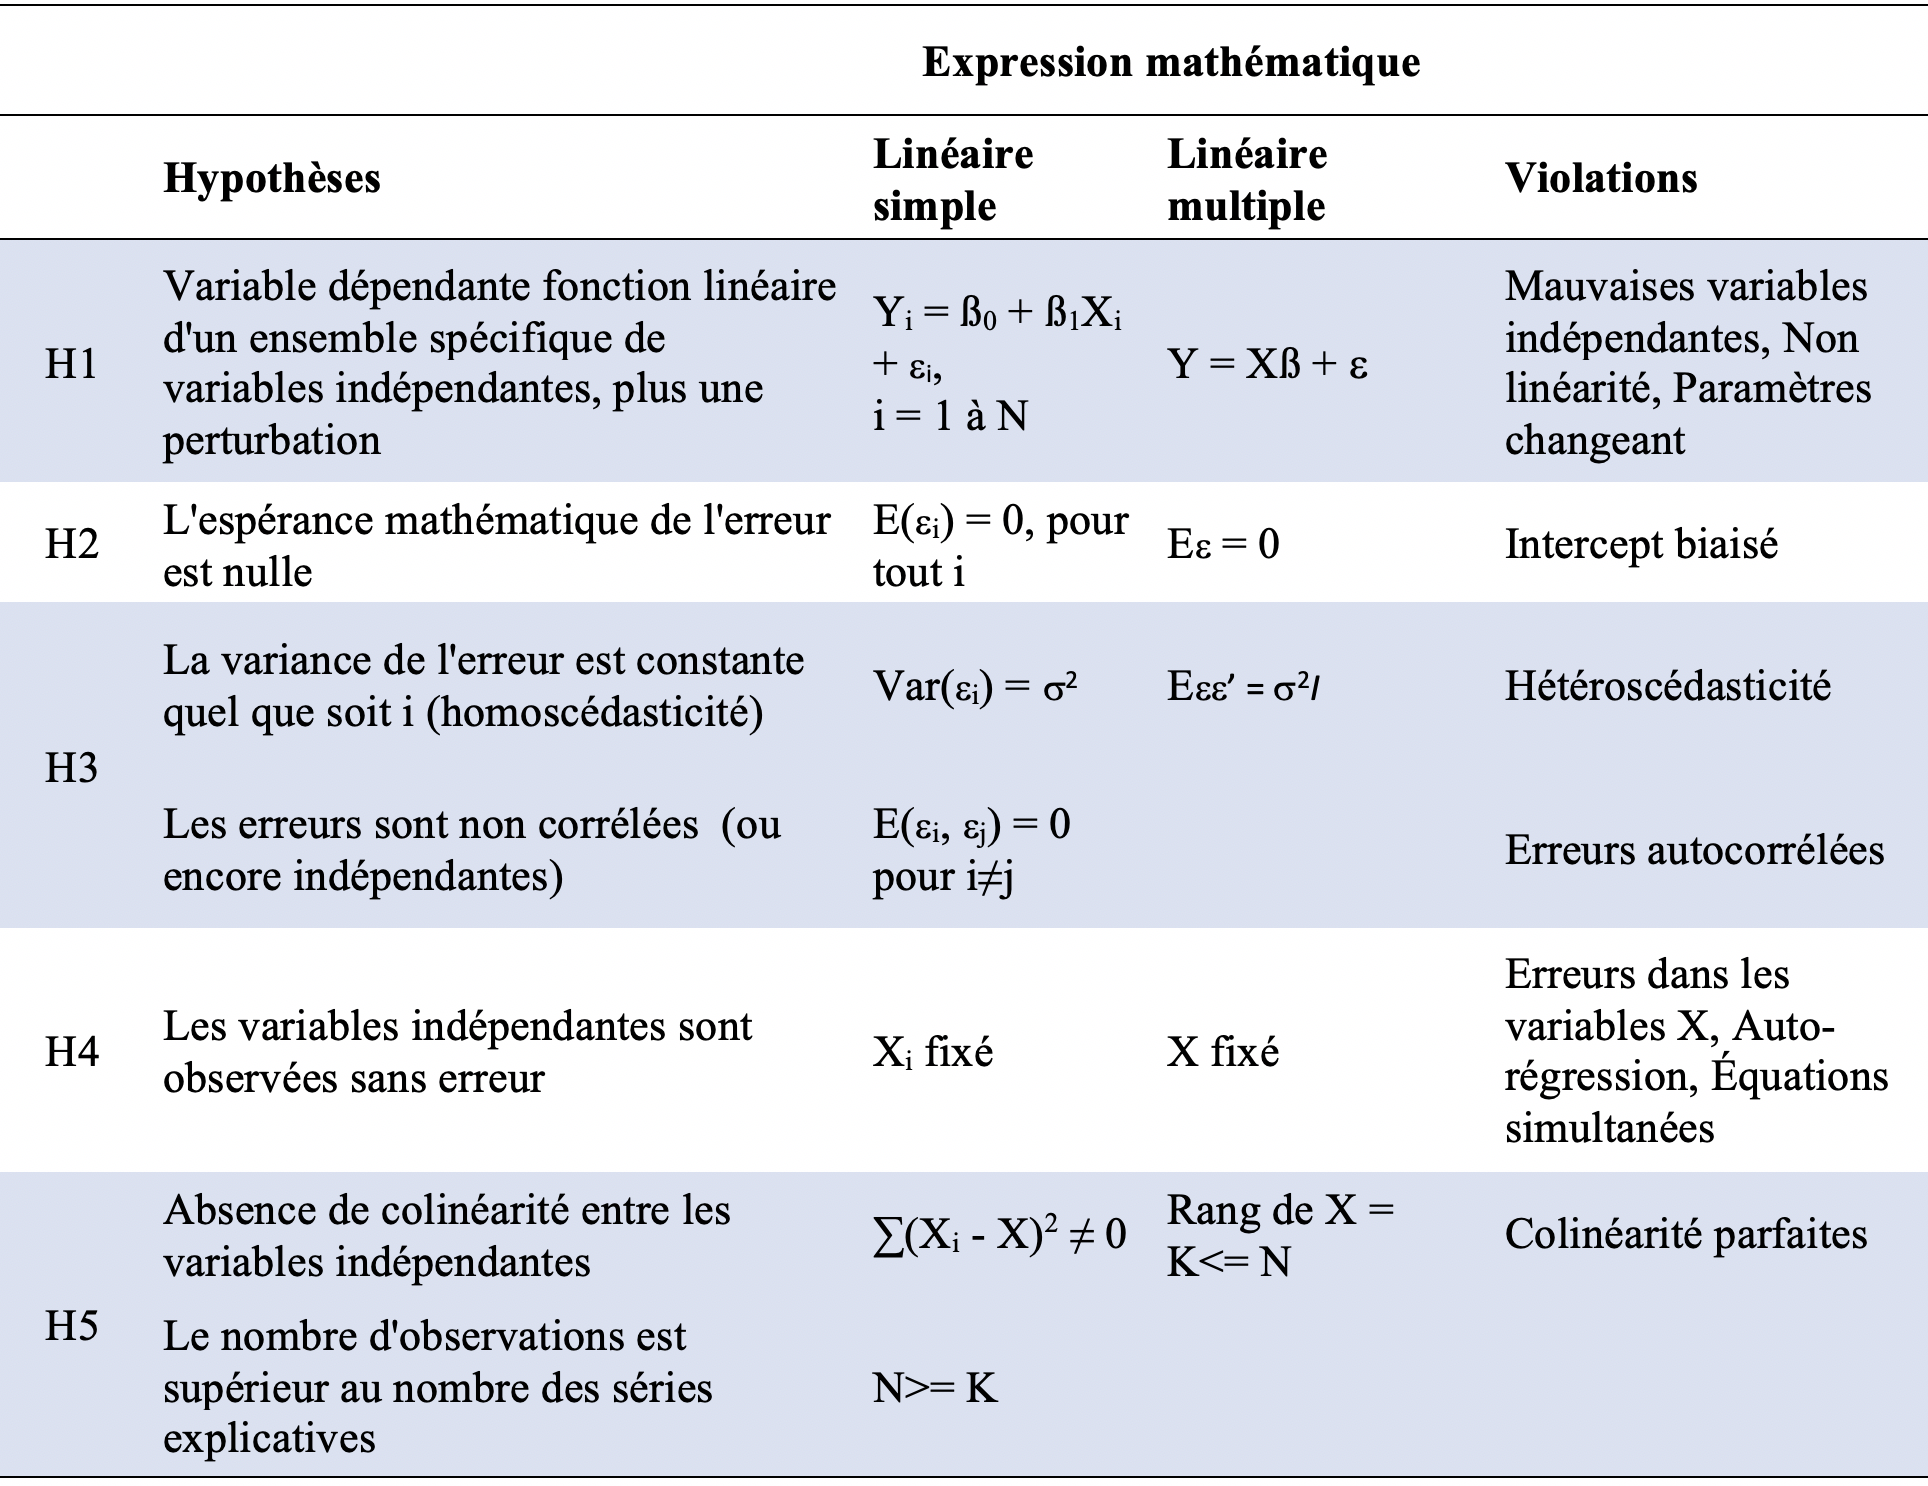
\includegraphics[width=26.78in]{/Users/visseho/OneDrive - UQAM/Cours/Images_cours/hypotheses_regression}

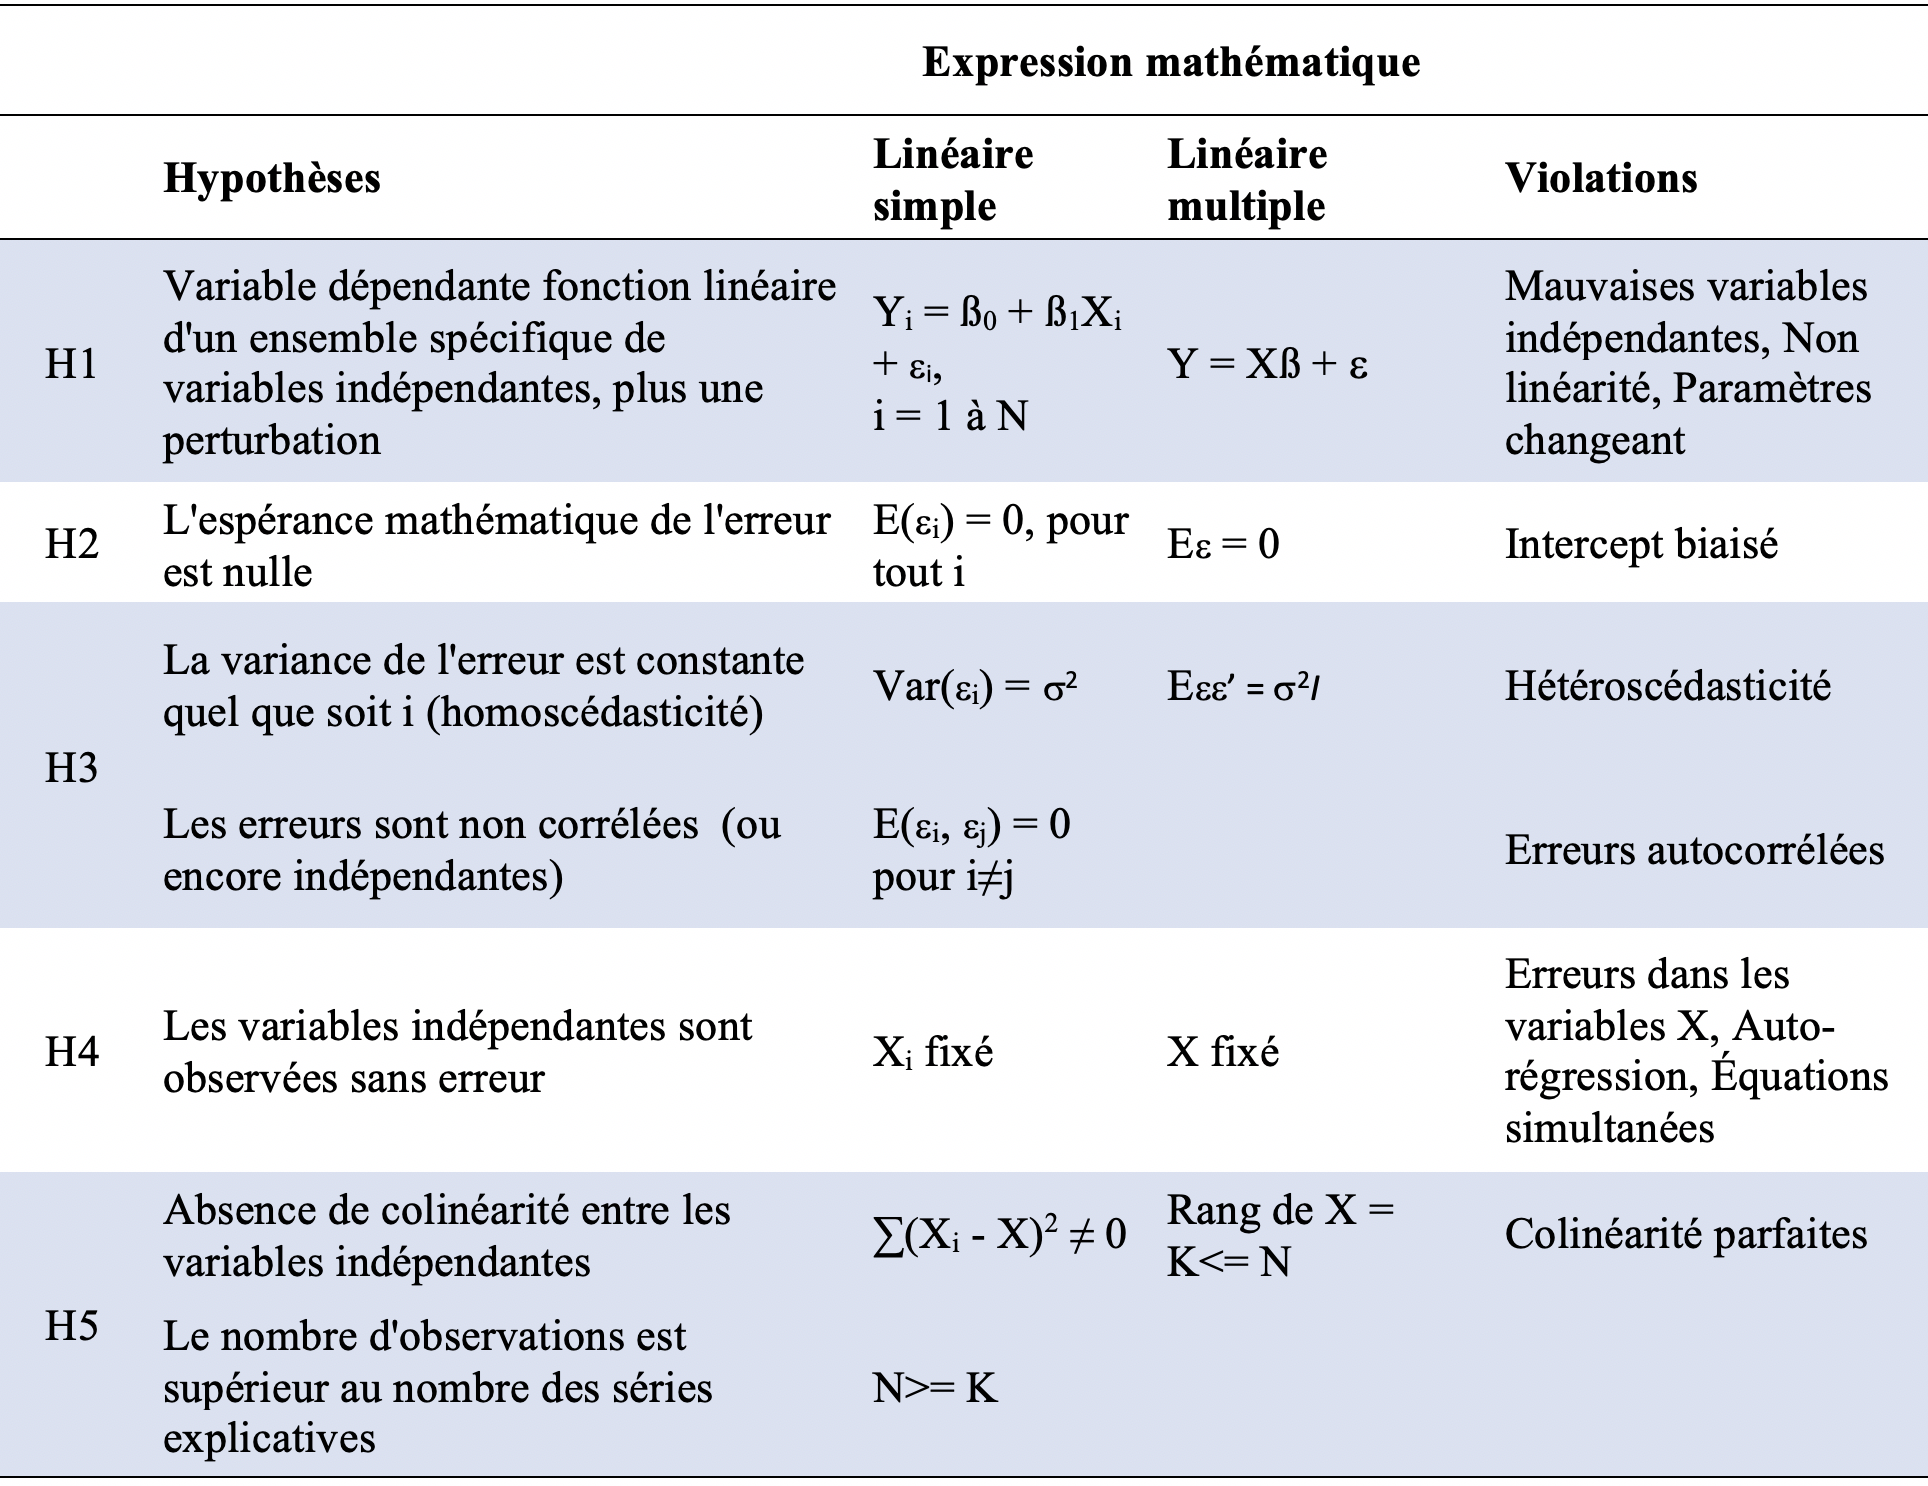
\includegraphics{/Users/visseho/OneDrive - UQAM/Cours/Images_cours/hypotheses_regression.png}

\hypertarget{moduxe8le-guxe9nuxe9ral}{%
\subsection{Modèle général}\label{moduxe8le-guxe9nuxe9ral}}

\begin{Shaded}
\begin{Highlighting}[]
\NormalTok{reg_mul2 <-}\StringTok{ }\KeywordTok{lm}\NormalTok{(beat_burnfood }\OperatorTok{~}\StringTok{ }\NormalTok{sec_school }\OperatorTok{+}\StringTok{ }\NormalTok{no_media }\OperatorTok{+}\StringTok{ }\NormalTok{region }\OperatorTok{+}\StringTok{ }\NormalTok{year_binaire, }\DataTypeTok{data =}\NormalTok{ dhs_ipv)}
\KeywordTok{summary}\NormalTok{(reg_mul2)}
\end{Highlighting}
\end{Shaded}

\begin{verbatim}
## 
## Call:
## lm(formula = beat_burnfood ~ sec_school + no_media + region + 
##     year_binaire, data = dhs_ipv)
## 
## Residuals:
##     Min      1Q  Median      3Q     Max 
## -17.862  -4.319  -0.565   4.439  25.216 
## 
## Coefficients:
##                                    Estimate Std. Error t value Pr(>|t|)    
## (Intercept)                         1.96534    4.34338   0.452   0.6518    
## sec_school                         -0.13231    0.07834  -1.689   0.0941 .  
## no_media                            0.36125    0.06505   5.553    2e-07 ***
## regionLatin America                -0.87767    3.23636  -0.271   0.7868    
## regionMiddle East and Central Asia  9.27064    3.74159   2.478   0.0148 *  
## regionSub-Saharan Africa            5.02288    2.82363   1.779   0.0780 .  
## year_binaireAvant 2010              2.84442    1.90333   1.494   0.1379    
## ---
## Signif. codes:  0 '***' 0.001 '**' 0.01 '*' 0.05 '.' 0.1 ' ' 1
## 
## Residual standard error: 9.262 on 109 degrees of freedom
##   (35 observations deleted due to missingness)
## Multiple R-squared:  0.5148, Adjusted R-squared:  0.4881 
## F-statistic: 19.28 on 6 and 109 DF,  p-value: 3.275e-15
\end{verbatim}

\hypertarget{combinons-les-ruxe9sultats}{%
\subsection{Combinons les résultats}\label{combinons-les-ruxe9sultats}}

\begin{itemize}
\tightlist
\item
  Le package stargazer est un excellent package que vous devez avoir
  dans votre boîte à outils R. Il permet de combiner plusieurs résultats
  de régression.
\end{itemize}

\begin{Shaded}
\begin{Highlighting}[]
\KeywordTok{library}\NormalTok{(stargazer)}
\end{Highlighting}
\end{Shaded}

\begin{verbatim}
## 
## Please cite as:
\end{verbatim}

\begin{verbatim}
##  Hlavac, Marek (2018). stargazer: Well-Formatted Regression and Summary Statistics Tables.
\end{verbatim}

\begin{verbatim}
##  R package version 5.2.2. https://CRAN.R-project.org/package=stargazer
\end{verbatim}

\url{https://cran.r-project.org/web/packages/stargazer/vignettes/stargazer.pdf}

\hypertarget{combinons-les-ruxe9sultats-1}{%
\subsection{Combinons les
résultats}\label{combinons-les-ruxe9sultats-1}}

\begin{Shaded}
\begin{Highlighting}[]
\KeywordTok{stargazer}\NormalTok{(reg1, reg2, reg_mul1, reg_mul2, }\DataTypeTok{title =} \StringTok{"Divers modèles"}\NormalTok{, }\DataTypeTok{align =} \OtherTok{TRUE}\NormalTok{, }\DataTypeTok{type =} \StringTok{"text"}\NormalTok{)}
\end{Highlighting}
\end{Shaded}

\begin{verbatim}
## 
## Divers modèles
## ==================================================================================================================================
##                                                                          Dependent variable:                                      
##                                    -----------------------------------------------------------------------------------------------
##                                                                             beat_burnfood                                         
##                                              (1)                     (2)                     (3)                     (4)          
## ----------------------------------------------------------------------------------------------------------------------------------
## sec_school                                -0.387***                                        -0.103                  -0.132*        
##                                            (0.066)                                         (0.072)                 (0.078)        
##                                                                                                                                   
## no_media                                                          0.414***                0.385***                0.361***        
##                                                                    (0.052)                 (0.059)                 (0.065)        
##                                                                                                                                   
## regionLatin America                                                                                                -0.878         
##                                                                                                                    (3.236)        
##                                                                                                                                   
## regionMiddle East and Central Asia                                                                                 9.271**        
##                                                                                                                    (3.742)        
##                                                                                                                                   
## regionSub-Saharan Africa                                                                                           5.023*         
##                                                                                                                    (2.824)        
##                                                                                                                                   
## year_binaireAvant 2010                                                                                              2.844         
##                                                                                                                    (1.903)        
##                                                                                                                                   
## Constant                                  24.070***                3.529**                 6.409**                  1.965         
##                                            (1.919)                 (1.773)                 (3.191)                 (4.343)        
##                                                                                                                                   
## ----------------------------------------------------------------------------------------------------------------------------------
## Observations                                 118                     118                     116                     116          
## R2                                          0.227                   0.356                   0.442                   0.515         
## Adjusted R2                                 0.220                   0.351                   0.432                   0.488         
## Residual Std. Error                   11.426 (df = 116)       10.867 (df = 116)       9.759 (df = 113)        9.262 (df = 109)    
## F Statistic                        33.998*** (df = 1; 116) 64.159*** (df = 1; 116) 44.674*** (df = 2; 113) 19.276*** (df = 6; 109)
## ==================================================================================================================================
## Note:                                                                                                  *p<0.1; **p<0.05; ***p<0.01
\end{verbatim}

\% Table created by stargazer v.5.2.2 by Marek Hlavac, Harvard
University. E-mail: hlavac at fas.harvard.edu \% Date and time: Thu, Jun
10, 2021 - 12:07:14 \% Requires LaTeX packages: dcolumn

\begin{table}[!htbp] \centering 
  \caption{Divers modèles} 
  \label{} 
\begin{tabular}{@{\extracolsep{5pt}}lD{.}{.}{-3} D{.}{.}{-3} D{.}{.}{-3} D{.}{.}{-3} } 
\\[-1.8ex]\hline 
\hline \\[-1.8ex] 
 & \multicolumn{4}{c}{\textit{Dependent variable:}} \\ 
\cline{2-5} 
\\[-1.8ex] & \multicolumn{4}{c}{beat\_burnfood} \\ 
\\[-1.8ex] & \multicolumn{1}{c}{(1)} & \multicolumn{1}{c}{(2)} & \multicolumn{1}{c}{(3)} & \multicolumn{1}{c}{(4)}\\ 
\hline \\[-1.8ex] 
 sec\_school & -0.387^{***} &  & -0.103 & -0.132^{*} \\ 
  & (0.066) &  & (0.072) & (0.078) \\ 
  & & & & \\ 
 no\_media &  & 0.414^{***} & 0.385^{***} & 0.361^{***} \\ 
  &  & (0.052) & (0.059) & (0.065) \\ 
  & & & & \\ 
 regionLatin America &  &  &  & -0.878 \\ 
  &  &  &  & (3.236) \\ 
  & & & & \\ 
 regionMiddle East and Central Asia &  &  &  & 9.271^{**} \\ 
  &  &  &  & (3.742) \\ 
  & & & & \\ 
 regionSub-Saharan Africa &  &  &  & 5.023^{*} \\ 
  &  &  &  & (2.824) \\ 
  & & & & \\ 
 year\_binaireAvant 2010 &  &  &  & 2.844 \\ 
  &  &  &  & (1.903) \\ 
  & & & & \\ 
 Constant & 24.070^{***} & 3.529^{**} & 6.409^{**} & 1.965 \\ 
  & (1.919) & (1.773) & (3.191) & (4.343) \\ 
  & & & & \\ 
\hline \\[-1.8ex] 
Observations & \multicolumn{1}{c}{118} & \multicolumn{1}{c}{118} & \multicolumn{1}{c}{116} & \multicolumn{1}{c}{116} \\ 
R$^{2}$ & \multicolumn{1}{c}{0.227} & \multicolumn{1}{c}{0.356} & \multicolumn{1}{c}{0.442} & \multicolumn{1}{c}{0.515} \\ 
Adjusted R$^{2}$ & \multicolumn{1}{c}{0.220} & \multicolumn{1}{c}{0.351} & \multicolumn{1}{c}{0.432} & \multicolumn{1}{c}{0.488} \\ 
Residual Std. Error & \multicolumn{1}{c}{11.426 (df = 116)} & \multicolumn{1}{c}{10.867 (df = 116)} & \multicolumn{1}{c}{9.759 (df = 113)} & \multicolumn{1}{c}{9.262 (df = 109)} \\ 
F Statistic & \multicolumn{1}{c}{33.998$^{***}$ (df = 1; 116)} & \multicolumn{1}{c}{64.159$^{***}$ (df = 1; 116)} & \multicolumn{1}{c}{44.674$^{***}$ (df = 2; 113)} & \multicolumn{1}{c}{19.276$^{***}$ (df = 6; 109)} \\ 
\hline 
\hline \\[-1.8ex] 
\textit{Note:}  & \multicolumn{4}{r}{$^{*}$p$<$0.1; $^{**}$p$<$0.05; $^{***}$p$<$0.01} \\ 
\end{tabular} 
\end{table}

\hypertarget{utilisation-du-package-broom}{%
\subsection{Utilisation du package
broom}\label{utilisation-du-package-broom}}

\begin{itemize}
\tightlist
\item
  Nécessaire pour réutiliser les données de la régression
\end{itemize}

\begin{Shaded}
\begin{Highlighting}[]
\KeywordTok{summary}\NormalTok{(reg_mul2)}
\end{Highlighting}
\end{Shaded}

\begin{verbatim}
## 
## Call:
## lm(formula = beat_burnfood ~ sec_school + no_media + region + 
##     year_binaire, data = dhs_ipv)
## 
## Residuals:
##     Min      1Q  Median      3Q     Max 
## -17.862  -4.319  -0.565   4.439  25.216 
## 
## Coefficients:
##                                    Estimate Std. Error t value Pr(>|t|)    
## (Intercept)                         1.96534    4.34338   0.452   0.6518    
## sec_school                         -0.13231    0.07834  -1.689   0.0941 .  
## no_media                            0.36125    0.06505   5.553    2e-07 ***
## regionLatin America                -0.87767    3.23636  -0.271   0.7868    
## regionMiddle East and Central Asia  9.27064    3.74159   2.478   0.0148 *  
## regionSub-Saharan Africa            5.02288    2.82363   1.779   0.0780 .  
## year_binaireAvant 2010              2.84442    1.90333   1.494   0.1379    
## ---
## Signif. codes:  0 '***' 0.001 '**' 0.01 '*' 0.05 '.' 0.1 ' ' 1
## 
## Residual standard error: 9.262 on 109 degrees of freedom
##   (35 observations deleted due to missingness)
## Multiple R-squared:  0.5148, Adjusted R-squared:  0.4881 
## F-statistic: 19.28 on 6 and 109 DF,  p-value: 3.275e-15
\end{verbatim}

\begin{Shaded}
\begin{Highlighting}[]
\NormalTok{result <-}\StringTok{ }\KeywordTok{summary}\NormalTok{(reg_mul2)}
\NormalTok{result}
\end{Highlighting}
\end{Shaded}

\begin{verbatim}
## 
## Call:
## lm(formula = beat_burnfood ~ sec_school + no_media + region + 
##     year_binaire, data = dhs_ipv)
## 
## Residuals:
##     Min      1Q  Median      3Q     Max 
## -17.862  -4.319  -0.565   4.439  25.216 
## 
## Coefficients:
##                                    Estimate Std. Error t value Pr(>|t|)    
## (Intercept)                         1.96534    4.34338   0.452   0.6518    
## sec_school                         -0.13231    0.07834  -1.689   0.0941 .  
## no_media                            0.36125    0.06505   5.553    2e-07 ***
## regionLatin America                -0.87767    3.23636  -0.271   0.7868    
## regionMiddle East and Central Asia  9.27064    3.74159   2.478   0.0148 *  
## regionSub-Saharan Africa            5.02288    2.82363   1.779   0.0780 .  
## year_binaireAvant 2010              2.84442    1.90333   1.494   0.1379    
## ---
## Signif. codes:  0 '***' 0.001 '**' 0.01 '*' 0.05 '.' 0.1 ' ' 1
## 
## Residual standard error: 9.262 on 109 degrees of freedom
##   (35 observations deleted due to missingness)
## Multiple R-squared:  0.5148, Adjusted R-squared:  0.4881 
## F-statistic: 19.28 on 6 and 109 DF,  p-value: 3.275e-15
\end{verbatim}

\begin{Shaded}
\begin{Highlighting}[]
\NormalTok{result[[}\DecValTok{1}\NormalTok{]][]}
\end{Highlighting}
\end{Shaded}

\begin{verbatim}
## lm(formula = beat_burnfood ~ sec_school + no_media + region + 
##     year_binaire, data = dhs_ipv)
\end{verbatim}

\hypertarget{tidy}{%
\subsection{Tidy}\label{tidy}}

\begin{itemize}
\tightlist
\item
  tidy
\item
  glance
\item
  augment
\end{itemize}

\begin{Shaded}
\begin{Highlighting}[]
\KeywordTok{tidy}\NormalTok{(reg_mul2)}
\end{Highlighting}
\end{Shaded}

\begin{verbatim}
## # A tibble: 7 x 5
##   term                               estimate std.error statistic     p.value
##   <chr>                                 <dbl>     <dbl>     <dbl>       <dbl>
## 1 (Intercept)                           1.97     4.34       0.452 0.652      
## 2 sec_school                           -0.132    0.0783    -1.69  0.0941     
## 3 no_media                              0.361    0.0651     5.55  0.000000200
## 4 regionLatin America                  -0.878    3.24      -0.271 0.787      
## 5 regionMiddle East and Central Asia    9.27     3.74       2.48  0.0148     
## 6 regionSub-Saharan Africa              5.02     2.82       1.78  0.0780     
## 7 year_binaireAvant 2010                2.84     1.90       1.49  0.138
\end{verbatim}

\begin{Shaded}
\begin{Highlighting}[]
\NormalTok{result1 <-}\StringTok{ }\KeywordTok{tidy}\NormalTok{(reg_mul2)}

\NormalTok{result1}\OperatorTok{$}\NormalTok{estimate[}\DecValTok{3}\NormalTok{]}
\end{Highlighting}
\end{Shaded}

\begin{verbatim}
## [1] 0.3612471
\end{verbatim}

\hypertarget{glance}{%
\subsection{Glance}\label{glance}}

\begin{Shaded}
\begin{Highlighting}[]
\KeywordTok{glance}\NormalTok{(reg_mul2)}
\end{Highlighting}
\end{Shaded}

\begin{verbatim}
## # A tibble: 1 x 12
##   r.squared adj.r.squared sigma statistic  p.value    df logLik   AIC   BIC
##       <dbl>         <dbl> <dbl>     <dbl>    <dbl> <dbl>  <dbl> <dbl> <dbl>
## 1     0.515         0.488  9.26      19.3 3.28e-15     6  -419.  854.  876.
## # ... with 3 more variables: deviance <dbl>, df.residual <int>, nobs <int>
\end{verbatim}

\begin{Shaded}
\begin{Highlighting}[]
\NormalTok{result2 <-}\StringTok{ }\KeywordTok{glance}\NormalTok{(reg_mul2)}
\end{Highlighting}
\end{Shaded}

\hypertarget{augment}{%
\subsection{Augment}\label{augment}}

\begin{Shaded}
\begin{Highlighting}[]
\KeywordTok{augment}\NormalTok{(reg_mul2)}
\end{Highlighting}
\end{Shaded}

\begin{verbatim}
## # A tibble: 116 x 12
##    .rownames beat_burnfood sec_school no_media region year_binaire .fitted
##    <chr>             <dbl>      <dbl>    <dbl> <chr>  <fct>          <dbl>
##  1 1                   4.4       25.2      1.5 Middl~ Avant 2010     11.3 
##  2 2                   4.9       67.7      8.7 Middl~ Avant 2010      8.27
##  3 3                   2.1       67.6      2.2 Middl~ Avant 2010      5.93
##  4 4                   0.3       46        6.4 Middl~ Avant 2010     10.3 
##  5 5                  12.1       74.6      7.4 Middl~ Avant 2010      6.88
##  6 8                   4.1       27.9     48.8 Asia   Apres 2010     15.9 
##  7 9                  29.2        7.7     33.2 Sub-S~ Avant 2010     20.8 
##  8 10                 19         10.2     38.8 Sub-S~ Avant 2010     22.5 
##  9 11                  6         14.3     45.7 Sub-S~ Apres 2010     21.6 
## 10 12                  5.4       20.8      8.4 Latin~ Avant 2010      4.21
## # ... with 106 more rows, and 5 more variables: .resid <dbl>, .hat <dbl>,
## #   .sigma <dbl>, .cooksd <dbl>, .std.resid <dbl>
\end{verbatim}

\end{document}
